
\section{Overview}
\label{sec:intro}
Modern web applications often use database engines to 
manage a large amount of user data, such as user profiles in social network applications and transaction
records in on-line shopping platforms~\cite{webapp}.  
The schema of such data goes through changes, such as table renaming, column
deletion, and others, for better performance or functionality when an application evolves \cite{wang2017verifying}.
Unfortunately, it is difficult for developers to keep their code 
consistent with database schema changes all the time, a task we
refer to as \textit{schema-related code refactoring}, with any inconsistency leading
to application crashes.

Schema-related refactoring and
traditional refactoring like class renaming share similarities, given that
popular Object Relational Mapping (ORM) frameworks, such as Rails \cite{rails},  
Django \cite{django}, and Hibernate \cite{hibernate},
allow database data to be
updated and retrieved in an object-oriented way---the name of a database table corresponds to the name of a model class
and the names of table columns are the same as class fields.

%\shan{TODO: we may need to expand the onebody example}
However, they also differ in various aspects, due to the unique nature of persistent data,
as we elaborate below\footnote{Our discussion generally applies to
all web applications developed upon ORM frameworks, although our
examples use Ruby on Rails applications.}.



%Comparing with traditional software, database-backed web applications face the unique code-maintenance challenge of making code changes consistent with database schema changes. Because web applications are often constructed using Object Relational Mapping (ORM) frameworks allowing the properties and relationships of the objects in an application to be easily stored and retrieved from a database in an object-oriented way, which can go beyond the form of class name and field name as used in traditional software, e.g.,  in line 2 in listing~\ref{onebody-query}, the \texttt{sequence} column of \texttt{people} table is used as a parameter of \texttt{order} function call in the form of string. 



% The class definition in database-backed web applications  will not explicitly declare its fields since database columns  will be mapped to the fields by ORM frameworks implicitly. 
% ORM frameworks will implicitly map database columns to the object's class. 
 


% \begin{lstlisting}[float=t,language=Ruby,label={onebody-query}, caption=Inconsistent code from Onebody]
% app/controllers/checkin/families_controller.rb
%     # select * from people where family_id = ? 
%     # and is_deleted = ? order by sequence
% 1   @family.people.undeleted.order('sequence')

% app/models/person.rb
% 2   person.sequence = 1
% \end{lstlisting}
% For example, in Spree \cite{spree}, an online-shopping application, a table named orders is used to 
% keep the order information. In one version, 
% developers renamed a column in this table from \texttt{guest\_token} to \texttt{token} since the column starts to store \texttt{tokens} used in login cookies for not only guest but also general users\shan{what does token mean? what does general token mean?}, it has to change all the references to the old name \texttt{guest\_token} to the new name \texttt{token}, which results in 284 lines of code change across 32 files. 
%It's challenging for developers to manually refactor the application code based on the schema change. 

\textit{How is schema defined?} Different from a regular class whose 
field names and field types are defined by its class
declaration, a model class's structure has to match its corresponding database table that is created once at an application's installation or upgrade.
%with its data retrieved into objects at run time.
In fact, in some ORM frameworks like Rails, persistent fields of a model class are \textit{not} declared in its class
definition and are instead automatically mapped by Rails from the corresponding table schema, which is 
%Consequently, although every table (e.g., \texttt{people}) corresponds to a class
%with a singularized name (e.g., \texttt{Person}), the schema, including table names, column
%names and types, and other information, has to be 
defined through ORM
APIs like \texttt{create\_table} in Rails or
\texttt{CreateModel} in Django in a type of files called
\textit{migration files},
as shown in Listing \ref{migration}. 
%In fact, the corresponding model class definition needs not contain definitions of column fields.

\textit{How is schema changed?} 
%One cannot change the
%schema (e.g., a column name) by changing the class definition. 
Schema changes are expressed
through ORM APIs in migration files (e.g., line 4 in Listing 
\ref{migration}
renames the column \texttt{sequence} in table \texttt{people}), 
which informs the web application about how to 
update its database during installation and upgrade.
In an ORM framework like Rails, schema changes cannot be seen in
class definitions.

\lstinputlisting[float=t, basicstyle=\footnotesize\ttfamily, label={migration}, caption={Migration files from Onebody},language=Ruby]{migration.rb}

\lstinputlisting[float=t,basicstyle=\footnotesize\ttfamily, label={onebody-query}, caption={Inconsistent code from Onebody},language=Ruby]{onebody-query.rb}

\textit{What code refactoring is needed?} Following a schema
change in the migration file, corresponding references in the
application need to change. Some of these are just
class or field renaming like in line 2 of Listing \ref{onebody-query}, while some require changing ORM APIs' parameters like in line 1 of Listing \ref{onebody-query}.
%and hence requires ORM knowledge.

For example, developers of Onebody~\cite{onebody}, a popular social network application, used 
a table \texttt{people} to keep user information. In one commit, they renamed the \texttt{sequence} column in \texttt{people} to \texttt{position} (line 4 in Listing \ref{migration}). In the same commit, they
correctly updated the reference to \texttt{sequence} in 6 places across 4 files like the one in line 2 of Listing \ref{onebody-query}, but forgot to change the other 5 places, 
such as the parameter reference shown in line 1 of Listing
\ref{onebody-query}. This inconsistency caused web users to
suffer from webpage crashes~\cite{onebodyissue672}.
%\url{https://github.com/seven1m/onebody/issues/672}}
%\shan{the issue report does not read like application crash.}

%https://github.com/spree/spree/pull/8826/files

% Moreover, the challenge is escalated by the prevalent usage of Object-Relational Mapping (ORM) frameworks, such as Ruby on Rails~\cite{rails}, Django for Python~\cite{django}, and Hibernate for Java~\cite{django}. Because they provide a convenient way for developers to evolve their database schema over time using object-oriented code without issuing `ALTER TABLE' SQL commands to database, which eases the efforts and results in more frequent schema change. 
% \shan{Do you have evidence that there are more frequent schema changes in ORM applications?
% If not, I don't think we can claim it. I can imagine maybe it is more error prone, because
% schema changes and declaration are in different files from files that use the tables and columns,
% so that it is more isolated ... I don't know ...} 
% \junwen{I have found that in an empirical study on web application not using ORM framework~\cite{qiu2013empirical}, the average schema change per release is 60, so we cannot draw the conclusion that orm schema changes faster. But their way of calculating change is to check every revision instead of every release. We may change our counting methodology and regenerate the result. 
% }


%TODO:\shan{There needs to be a clearer definition of what are code-schema inconsistencies.}
%TODO:\shan{can some of the inconsistency get exposed by unit testing? }
% Inconsistency between application code and its data schema could cause web-page crashes 
% with database exceptions thrown 
% Different from traditional software, the object class's fields in database-backed web applications are not declared explicitly in the class itself but mapped to the database columns by ORM frameworks implicitly
 
% Thus, existing refactoring tools that tackle method or field renaming are not able to refactor the database-backed web applications.

Recent work motivated tool support for schema-related refactoring  \cite{wang2017verifying} and proposed techniques to synthesize updates to a list of 
SQL queries given the old schema and the new schema written in SQL
\cite{wang2019synthesizing}. Although inspiring, it does not directly help
many web applications, whose schema changes
and database operations are expressed in ORM APIs, rarely if ever in raw SQL.

%As a result, cross-stack analysis which combines the database information with application code is necessary to detect and fix the inconsistency  between application code and schema change. 
%Existing work MIGRATOR~\cite{wang2019synthesizing} can automatically synthesize database program after schema refactor, however it can only work on database programs written in SQL. 
% Also, MIGRATOR is guessing value correspondence from the name of table and column of two schema\shan{I don't understand}, which is possible to cause inaccurate mapping and generate incorrect refactoring. Also, MIGRATOR is not able to handle deletion change. \shan{I don't understand.} 



This paper presents {}, a tool that uses ORM-aware static analysis to help schema-related code refactoring in web applications
written in Rails \cite{rails} and Django \cite{django}, two popular web frameworks.
%\shan{can we say 'most' popular? can we say web application frameworks, instead of ORM frameworks to make it sound more general?}. \junwen{According to the data \url{https://www.statista.com/statistics/1124699/worldwide-developer-survey-most-used-frameworks-web/}, Django and Rails are not the most popular web app frameworks. But based on data we collected on github before, for apps with more than 100 starts, the most popular is Rails and then django}
Given two versions of a web application, 
\ETool{} analyzes and identifies schema changes from
migration files, searches for
any code inconsistent with the new schema,
and generates warnings and patches accordingly. %\shan{Why do we need the old code version? If I just give you one version,can you identify code--schema inconsistency?} \junwen{Yes, we can. Having the old version schema is to just make the detection even faster by only checking on the changed schema}.

%As an IDE plugin, \ETool{} supports two usage scenarios: 1) it can semi-automate \shan{why semi? what is not automated?} the refactoring for an old application after users make data-schema changes \shan{what type of data schema changes do you support? What is the scope/limitations of your tool?}. 2) it can identify remaining inconsistency between the data schema and the application code, after
%developers commit changes to both data schema and the application code.  %\shan{I can imagine two potential uses of this type of tools: (1) once a data schema change is made, it will help automate or semi-automate all the needed code changes; (2) given a data schema change AND changed software, it checks if there are inconsistency between the data schema and the software. Does your tool only offer functionality-2? Or do you offer both? I guess you offer both, if so, you should rephrase the usage flow and functionality description of your tool.} 
%This work makes the following contributions:


%\shan{What type of guarantees you can offer here? Do you guarantee that you will generate perfectly correct and complete refactoring?} 

To ease its adoption, we have integrated \ETool into the popular 
Visual Studio Code IDE~\cite{vscodepop} as a plugin. Web developers can use this plugin to
guide their schema-related refactoring or to look for
schema--code inconsistency bugs.

In our evaluation with 12 popular Rails and Django applications, 
\ETool detected \numRailsError schema--code inconsistencies 
%in 72 files 
caused by 35 schema changes in the past.
%and 25 warnings caused by 4 schema changes in application code that are caused by schema changes.  Among the 80 errors, 
We have reported 11 of them that exist in the latest versions to developers,
and got 10 of them already confirmed and 6 of them already patched based on
our suggestion.
Our examination of the rest \numFixed inconsistencies shows that 
they took many days for developers
to discover and fix.
%they took 378 days and 3 days on average for Rails and Django developers to discover and fix, respectively. %Moreover, \numfixedafterrelease of them are fixed after the version release. 

\ETool's source code is on Github~\cite{sourcecode} and the plugin can be downloaded from Visual Studio Marketplace~\cite{vscodemarketplace}.

\section{Background and Extended Motivation}
\label{sec:back}

\textbf{Background.} 
%ORM frameworks offer a \textit{migration} mechanism to consistently alter the database schema over time. 
A web application's schema gets initialized and 
updated by \textit{migration APIs} in migration 
files, a mechanism supported by ORM frameworks. 
For example, Listing \ref{migration} illustrates
two migration files, each with one migration API
call: the first creates a table named \texttt{people} with two columns \texttt{id} and \texttt{sequence},
which are automatically mapped to two fields in a corresponding model class
with a singular name
(\texttt{Person} class); the second 
renames a table column, which automatically causes
a field name change in its model class. 

During an installation/upgrade of a 
web application, the ORM framework executes all the
latest migration files not yet executed
on this installation, calling migration APIs in these files one by one and updating the schema along the way.
%; an existing installation will only execute the latest migration entry upon its software upgrade.

%\lstinputlisting[basicstyle=\footnotesize\ttfamily, label={migration}, caption={Inconsistent code from Onebody},language=Ruby]{migration.rb}

 
% Please add the following required packages to your document preamble:
% \usepackage{multirow}
%\label{change}


%Schema changes include addition, deletion, renaming on table, column, association, index, and constraint, and type change on association and column. For example, a column could change from a `int' type to a `string' type. And an association could change from `has\_one' to `has\_many'.  

\textbf{Extended motivation.}
A recent study~\cite{wang2017verifying} on 100 Rails applications 
%with more than 400 commits 
showed that most applications went through many schema changes.
%are common: about 28 per application on average.
%database schema has been changed at least once in all these 100 applications, with the average 
%about 28 schema changes on average over each application's life time.  
For further motivation, we studied
12 Rails and Django web applications from different categories like forum, e-commerce, social network, etc. \footnote{The application list is in our code
repository.} They are all highly rated, each with
more than 1000 stars on GitHub, 11,000--900,000 lines of code and 500--100,000 commits. 


% Schema change could happen on table, columns, associations, and indices
% % \junwen{Isil's group also shows constraints change, we didn't since it's covered in previous paper and will not cause query issue}; 
% a change could be addition, deletion, renaming. Besides, for column and association, it also contains type change. For example, a column could change from a `int' type to a `string' type. And an association could change from `has\_one' to `has\_many'. 
% \begin{table}[]
\caption{Application Corpus}
\label{tab:apps}
\resizebox{1\columnwidth}{!}{
\begin{tabular}{llrrrr}
\hline
\hline
Name & Category & \# stars & \# commits & \# versions & \# loc \\
\hline
Lobsters & Forum & 3k & 2.1k & 19 & 11 k \\
Gitlab & Collaboration & 22.6k & 100k & 1040 & 932k \\
Spree & E-commerce & 11.3k & 23.4k & 244 & 74k \\
Tracks & Management & 1k & 4.4k & 19 & 16k \\
Diaspora & Social Network & 12.7k & 20k & 82 & 83k \\
Onebody & Social Network & 1.4k & 5.2k & 32 & 103k \\
\hline
Zulip &  Collaboration & 13.7k  & 42.5k & 78 & 162k \\
Awx & Management & 9.7k & 29.7k & 45 & 93k \\
Saleor & E-commerce & 11.1k & 18.5k & 142 & 174k \\
Healthchecks & Management & 3.8k & 1.7k & 26 & 17k \\
Gerapy & Management  & 2.4k & 0.5k & 26 & 22k \\
Posthog &  Collaboration & 4.1k & 3.1k & 52 & 39k \\
\hline
\hline
\end{tabular}
}
\end{table}

\textit{How often are schema changes?} 18\% -- 85\% of application versions
contain at least one schema change, and there are more than 8 changes for every
version on average.
Furthermore, changes are common throughout the development history of each
application. For example, across the 6 Rails applications, the most recent 25\%
of commits happen to contain about 25\% of all the schema
changes in total.

%, as shown in Table~\ref{tab:change-stat}.
%Note that, for all  applications except for Lobsters \cite{lobsters}, we treat every public code release as a version; since Lobsters does not specify code release/version, we treat every 100 code commits as one version. 

\textit{What types of changes are there?} As shown in Table \ref{tab:change-stat},
 changes to various aspects of the schema
 %tables, columns, association relationships (e.g., `has\_one'
%or `has\_many' relationship between two tables), and table indices, 
are all common.
About three quarters of changes add tables, columns, or indices, and
do not directly cause inconsistency with existing code. The remaining
one quarter of changes modify or delete existing tables, columns,
associations, or indices, immediately threatening code consistency, and hence
are the target of \ETool, as detailed
in Table \ref{tab:overview}.


\iffalse 
\textbf{How schema changes vary with age?} We split every application' history into four quarters, each with the same number of releases/versions and count the average number of schema changes in each quarter (time gaps between code releases
are stable within each application). As shown in Figure~\ref{fig:evo-time}, although there are more changes in the first two quarters, changes in the latter two quarters
are still common.
%, indicating that schema-related refactoring is necessary for applications at any development stage no matter it's new or mature. 
%\shan{If you want to save space, you can replace Figure 1 with a text explanation saying how many changes are there in each major version: I assume there are 13 major versions for AWX? Based on AWX, I feel there are indeed more schema changes at the beginning, but there are still a good amount of changes lat j er on. That is probably a more fair claim.}


\begin{figure}
    \centering
    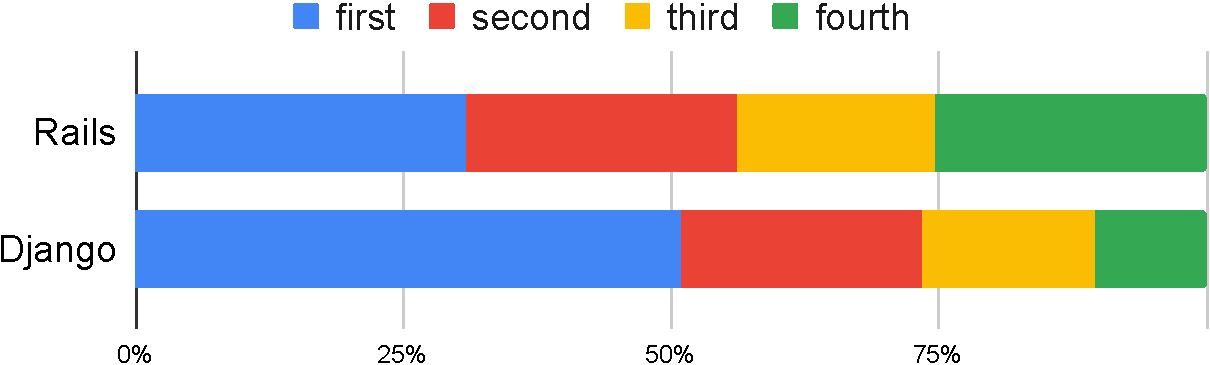
\includegraphics[width=\columnwidth]{figs/breakdown-4.pdf}
    \caption{Quarter Breakdown of Schema Changes (Aggregated View)}
    \label{fig:evo-time}
\end{figure}
% \shan{Explain how is your study different from that by
% Isil's group. It is also fine if your study is similar
% with Isil's group's study, and just that you look at different sets of applications. No matter what is the case, please explain clearly.}
\fi 


% \shan{need to introduce these applications a bit. why you choose these applications to study; how large they are; how long they have been under development, etc.}

%Overall, schema changes of various types broadly exist in applications across their development phases. Related refactoring support will be broadly beneficial.






\begin{table}
\caption{Number of Schema Changes per Version}
\label{tab:change-stat}
\centering
%\setlength{\tabcolsep}{2pt} 
%\resizebox{\columnwidth}{!}{
\begin{tabular}{lrrrrr}
\arrayrulecolor{black}\hline  
\arrayrulecolor{black}\hline
Change Target  & Table  & Column  & Association  & Index  & Total \\
\arrayrulecolor{black}\hline
Django & 1.0           & 4.4            & 2.6                & 0.2     & 8.2      \\
Rails  & 1.6           & 4.8            & 2.2                & 1.3  & 9.9     \\   
\arrayrulecolor{black}\hline  
\arrayrulecolor{black}\hline
\end{tabular}
% \begin{tabular}{l|rr}

% \arrayrulecolor{black}\hline  
% \arrayrulecolor{black}\hline
% Types & Django  &  Rails \\ \hline
% Table Changes & 1.1 & 1.6 \\
% Column Changes & 4.7 & 4.8 \\
% Association Change & 2.5 & 2.2 \\
% Index Changes & 0.1 & 1.3 \\ 
% \hline
% Total & 8.4 & 9.8 \\

% \arrayrulecolor{black}\hline  
% \arrayrulecolor{black}\hline
% \end{tabular}
%}
\end{table}






\section{Approach}
\label{sec:approach}
This section discusses how \ETool conducts inconsistency checking and refactoring
step by step, based on the source code of 
two versions of an application.
Unless specially explained,
the code analysis is based on
AST trees generated by Yard \cite{yard} for Rails
 and 
pyast \cite{pyparser} for Django programs.
\subsection{Schema change extraction}
\label{subsec:schema-change-extraction}
% \paragraph{\textbf{Schema extraction}}
Different from previous work~\cite{wang2019synthesizing} that identifies schema changes by comparing the old and the new schemas written in SQL,
\Tool takes the unique opportunity offered by
web applications and identifies schema changes directly from all the new migration
files in the new version.
%offer the unique opportunity to extract schema changes directly from migration files, where schema changes
% are explicitly listed in order. 
%  The migration file works as a `diff' to the schema file. In one commit, developers can write as many as migration files to change their schema.  

% Taking this unique opportunity, \Tool{} analyzes newly added migration files between two versions one by one.
Specifically, 12 out of 19 Rails migration APIs and 6 out of 17 Django
migration APIs introduce schema changes that can immediately cause code inconsistency.
 \Tool{} matches each such API, or an API--parameter combination in case of Django, with one change type listed
 in Table \ref{tab:overview}. Whenever such an API call
 is identified in a migration file, \Tool{} extracts
 related change information, like table and column
 names, and saves it as a change
 record for later use.
 %Note that, one migration API call may introduce more
 %than one change record, like multiple columns getting
 %deleted using one \texttt{remove\_column} API call.
 %into a hash table for later use. In this hash table, the key represents the change type, and the value represents the previous and current schema.  
 %For example, line 5 in Listing~\ref{onebody-query} is extracted as  (Person.sequence, ``column\_rename'', Person.position). 
 \Tool aggregates related changes to the
 same target:  
deleting a column and then adding it back to the same table will be aggregated
and correctly considered as no change.
 

 %\shan{is there a special migration file for Django application? how exactly do you extract the scheme? do you use an existing framework to extract abstract syntax tree (AST) or something? in what form is the extracted schema represented for your later cross-version comparison? you may want to show an example} 
%  construct the enhanced schema \shan{what does enhanced mean?} from the abstract syntax tree (AST) generated by existing parser (yard for Rails applications, and pyparser for Django applications). The enhanced schema not only contains the tables and columns information but also preserves all the history information such as whether the current column is renamed from a previous column\shan{``all'' the history information sounds like you track all the changes since the 
%  creation of a table. I guess that is not the case? Does each version has its own migration file?
%  Or does every pair of code versions contain one migration file? Readers need some background
%  here.}. \Tool will also go through all the model class files \shan{what is the relationship
%  between these files and schema files?} to map the model classes to the tables. The mapping is built upon string transformation, for example, the \texttt{User} class maps to \texttt{users} table. 

Finally, in Rails, since an association relationship
is defined 
%partly through migration files  and 
partly through 
model classes, \Tool compares model class definitions, in addition to migration files, to get association changes. For example, the model class definitions in Listing \ref{association}
uses \texttt{has\_many} to indicate that each \texttt{User} record
is related to multiple \texttt{Comment} records, which can be retrieved through the association field \texttt{comments} defined in  \texttt{User}.

%\junwen{Also, for an association, such as one to many relation between \texttt{User} class and \texttt{Comment} class,  the foreign key \texttt{user\_id} is declared in migration files but the association type (has\_many/belongs\_to) and name (comments/user) is stored in the model class as shown in  Listing~\ref{association}.} 
%  \shan{?? what does this mean?}. The association type and association name are declared in the model class files as shown in Listing~\ref{associationfile}. So \Tool will analyze the association definition function such as \texttt{has\_many} in Rails (ForeignKey in Django) to extract association information.
%  \shan{you also mentioned index changes earlier. Do you identify that information here?}
%  \shan{It is not clear to me whether you try to extract all data schemas here, or you just
%  try to identify all the changed schema, and it is not clear whether you are just analyzing
%  one version of the software or both the old and the new versions.
%  This became clear after I read the next paragraph, but it should have been made clear
%  earlier.}
 
 
%  \paragraph{\textbf{Change extraction}}
%  By comparing the enhanced schema across two versions, \Tool{} is able to extract the schema change described in Section~\ref{change} into a hash table, where the key represents the change type, and the value represents the previous and current schema.  For example, the rename in line 1 in Listing~\ref{onebody-query} will be represented as \{``column\_rename'' : (Person.sequence, Person.position)\}. 
 
%  \shan{doesn't migration file like the one in Listing 1 already tell you what is been changed?
%  why do you need to compare schemas from two versions to know that?} \junwen{Ideally yes, but it's possible the migration file itself will be changed by developers.}
 
%\Tool{} first extracts the schema of the previous version of the application, and then extracts the schema of the current version of the application. Then, \Tool{} extracts the difference between the two schemas, where that schema difference is then compared with the queries in the current application to find any inconsistencies.

% \lstinputlisting[label={migrationfile}, caption={Migration file from Lobsters},language=Ruby]{migration.rb}


\subsection{Query extraction}
Next, \Tool identifies all the queries that can be
issued by the new version of the application.
%, together with source-code location,
%the table, column, association, and index information for each query if applicable.
%extraction takes the application's source code as the input and returns a set of code snippets that will issue queries and the corresponding tables, columns, associations, indices used as well as the location including filename, line of code, start offset, and length.
In ORM, a query can be expressed in two forms: 1) an ORM query API such as
\texttt{find\_by} in Rails and \texttt{filter} in Django invoked upon either
an object holding a previous query's result
or a model class like that in
line 1 of Listing~\ref{queries};
2) the reference to a model class' association field. For example, 
following the association definition in Listing \ref{association}, \texttt{@user.comments} in Listing \ref{queries}
issues a query to select records from table 
\texttt{comments} as `select * from comments where user\_id = user.id'. 
%an unchained one or chained one
%The query extraction will identify (1) unchained queries which are statements that start with model class name such as \texttt{User} and follow by query keywords such as line 1 in  Listing~\ref{queries}  (2) chained queries which are statements that start with variables which are query result and follow by query keywords such as line 2 in Listing~\ref{queries}. 

%There are two types of query keywords for a variable 

% (2) the association of the variable's class e.g., 
%, where  the class of @user and the class of comments are associated model classes.    

\Tool identifies both forms of queries
and extracts the names
of table, column, index, and related association information from each query. The analysis for Django applications is done by
analyzing the AST generated by pyast. 
The analysis
for Rails applications is 
built upon ORM-aware static analysis framework  PowerStation~\cite{yang2018powerstation}. 
%Also, it has a set of Django query API manually extracted from Django documents as part of the query keywords. 
%To identify chained queries (i.e., the query
%API or the association field is upon an object holding
%results from a previous query), 
\Tool uses intra-procedural dependency analysis to identify objects that hold results from a previous query.
In theory, it may miss queries on objects defined
in a different procedure.%, which is very rare in web applications.


\lstinputlisting[
float=t,
basicstyle=\footnotesize\ttfamily\color{black},
label={association}, 
caption={Association-Field Definition and Changes in Onebody},
language=Ruby]{association.rb}

\lstinputlisting[float=t,label={queries}, caption={Two types of statements that issue SQL queries},language=Ruby]{evolutionsaver/query.rb}

% \paragraph{\textbf{Extracting unchained queries}} \Tool starts the extraction from unchained queries, which are statements that start with model class name such as \texttt{User} and follows by query keywords such as \texttt{find\_by} in Rails, \texttt{filter} in Django. To identify the unchained query, \Tool will examine each function call node from the AST, and check whether the caller matches any model class name extracted in Section~\ref{subsec:schema-change-extraction} and the function name matches any query keywords\shan{how many keywords are there? how do you get
% a complete list of these keywords? are they complete? could there be false positives or negatives?}. If so, the node will be considered as an unchained query, and the variable it defines (@user in listing~\ref{queries}) will be kept for later usage including the name of the variable, and the table it queries on.

% \paragraph{\textbf{Extracting chained queries}} After getting a list of variables 
% \shan{1. what if this variable's value is assigned to another variable and then
% chained queries are issued on that variables? 2. is there any alias issue for variables?
% do you do these searches within one function? within one file?}
% defined by the unchained queries, denoted as query results, \Tool then still analyze all the function call nodes to see whether the caller is a variable from the query results, if so we will check the function name. Different from unchained queries,  the function name could be a query keyword, a column name of the model class, or an association of the model class. As shown in line 2 in  Listing~\ref{queries}, \texttt{comments} is an association of \texttt{User} class. \shan{why do you not need to worry about these for unchained queries?}\shan{do you keep looking for such chained queries or do you have a threshold
% of certain number of chains to check?}
% \shan{please comment on how common are chained queries}


% \paragraph{\textbf{Extracting tables, columns, associations in a query}}
% Besides the table name extracted from unchained queries, and the column name and association name extracted from the chained queries. We still need to analyze the parameters of the query functions to extract further information. For most of the query functions, the parameters are the column names of the queried tables, such as \texttt{name:?} in line in in Listing~\ref{queries}. It's also possible to use the associations as the parameter of query function such as \texttt{@user.includes(:comments)}. \Tool will extract the columns and associations used in the parameters for different query functions. 

% \shan{this paragraph is too long. you probably want to split the discussion about extracting non-chained queries from that about extracting chained queries.}
% \Tool{} extracts intraprocedural chained and unchained queries, as well as WRITE and READ queries. READ queries can be both chained and unchained. WRITE queries can only be unchained because WRITE queries do not return a QuerySet that can be further queried. Extracting WRITE queries is a very different process than extracting READ queries, as both the function and format of a WRITE and READ query are different. \Tool{} uses the python module AST to extract the table and/or column(s) that a specific WRITE query or unchained READ query refers to\shan{how do you know what statements are queries? is there a list of APIs that are read and a list of APIs that are read?}
% \shan{several topics are mixed here: (1) extracting queries; (2) extacting chained queries; (3) extracting table and column related to a query. you may want to split them to different paragraphs with each paragraph holding just one topic.}.\shan{you didn't identify association and index. should you mention that? Maybe you should organize all these by saying you will explain how to extract query statement and then explain how to identify key components of a query, including table name, column name, association, and index that are subject to potential inconsistencies.}\shan{an example can help.} The tables and columns are saved in a separate file. For chained queries, \Tool{} uses a variable system because initially for chained queries an unchained query is assigned to a variable. This variable is saved with the table that its assigned unchained query refers to in a separate file. When \Tool{} finds chained READ queries, queries in the format variable.method(column=value), \Tool{} goes through the saved variables and extracts the table and/or column(s) the query refers to and saves that information in a separate file. Another aspect to extracting queries is the case of extracting chaining queries where a query takes the “initial QuerySet of all entries in the database” [cite, not sure how?] applies a QuerySet method to that QuerySet, which returns another QuerySet, and then to that QuerySet another QuerySet method is applied. For example a chaining query could be in the format of Table.objects.filter(column=value).exclude(column=value). With chaining queries \Tool{} has to, like with chained queries, save the table to which the first method applies to, and, then, when \Tool{} recursively goes through the chaining query, \Tool{} finds the last saved table and that last saved table is the table to which the later QuerySet methods refer. Some lines of code are identified as WRITE or READ queries even if they are not. However, the extra “queries” counted do not matter, as all the WRITE and READ queries in the application are counted, and queries that improperly refer to a table or column in the schema are identified. Once \Tool{} saves all the query information in a separate file, \Tool{} sees if any of those queries are inconsistent with the new schema changes. \Tool{} also notifies if a query benefits from an added index, or if it does not benefit anymore from an index that has been deleted. 


\subsection{Inconsistency detection and refactoring suggestion}  
Finally, 
\Tool{} goes through each schema change, searches for inconsistency with
 queries in the new version, and generates refactoring suggestion accordingly
 (Table \ref{tab:overview}).

%And then we check whether the involved tables, columns, associations exist in the changed schema hash table. If we find a match, then we consider the application code needs to be refactored. If the columns referenced by a query match to a deleted indices, we consider the query might slow down. 

%\shan{I still don't get what exactly is the difference between what you are doing for renaming and traditional class/field name change refactoring. I can see that you definitely need an ORM-specific way to detect the name change. However, once you know that a class/field name should be changed, can you tell me what exactly is different from a traditional refactoring? 
% \url{https://www.jetbrains.com/help/idea/rename-refactorings.html\#rename_class_example},
% \url{https://docs.microsoft.com/en-us/visualstudio/ide/class-designer/refactoring-classes-and-types?view=vs-2019}}

\textbf{Name changes.} 
For the renaming of a table, \Tool{} checks if 
the old name \texttt{T}$_{{old}}$ is used in queries
from the new version\footnote{\Tool would issue false positives if 
\texttt{T}$_{old}$ is used to name another
table, which we have never observed.}; for the renaming of a column 
(e.g., Line 4 in Listing \ref{migration})
or an 
association field (e.g., Listing \ref{association}) \texttt{C}$_{{old}}$ in
a table \texttt{T}, \Tool checks if any new version's query refers to  
\texttt{C}$_{{old}}$ in \texttt{T}. Any such inconsistency is reported and
\Tool suggests the refactoring to replace the old name with the new name in
corresponding queries.
 
\begin{table}[t]
\caption{Schema Changes Handled by \Tool}
\label{tab:overview}
\centering
%\resizebox{\columnwidth}{!}{
\begin{tabular}{lll}
\arrayrulecolor{black}\hline  
\arrayrulecolor{black}\hline
Changes & Change Target &  \Tool{} Output\\
\arrayrulecolor{gray} \hline
\multirow{3}{*}{Name Change}   & Table & \multirow{3}{*}{Refactoring suggestion}  \\
\arrayrulecolor{gray} \cline{2-2}
 & Column  &  \\
 \arrayrulecolor{gray} \cline{2-2}
  & Association  &  \\
\arrayrulecolor{gray} \hline
\multirow{4}{*}{Deletion}   & Table &  Inconsistency error reports \\
\arrayrulecolor{gray} \cline{2-3}
 & Column  &  \multirow{2}{*}{Refactoring suggestion}\\
 \arrayrulecolor{gray} \cline{2-2}
  & Association  &  \\
\arrayrulecolor{gray} \cline{2-3}
  & Index  & Inconsistency warning \\
\arrayrulecolor{gray} \hline
\multirow{2}{*}{Type Change}   & Column & Inconsistency warning  \\
\arrayrulecolor{gray} \cline{2-3}
  & Association  & Partial refactoring suggestion\\
\arrayrulecolor{gray} \hline
\arrayrulecolor{black}\hline  
\arrayrulecolor{black}\hline
\end{tabular}

%}
\end{table}


\textbf{Deletion.} 
When a table \texttt{T}$_{old}$ is deleted, 
\Tool checks if  \texttt{T}$_{old}$ is still used in any query. If so, the query is 
reported as an error, with all the
statements in the same procedure that have control or data dependency on it 
highlighted. Since a table deletion is typically followed by major 
functionality changes, no refactoring attempt is made here. %\junwen{Posthog-3061~\cite{posthog-3061} is one pull request accepted by developers.}


When a column or association \texttt{C} in a table \texttt{T} is deleted, 
\Tool{} identifies any query that refers to \texttt{C} in \texttt{T} as an error.
In its refactoring attempt, \Tool removes \texttt{C} from
the query and runs the parser to see if the resulting query is valid.
If valid, a refactoring suggestion is made; otherwise, \Tool
reports this error without refactoring suggestion.  
%\junwen{Zulip-16975~\cite{zulip-16975} is one pull request for column deletion accepted by developers.}
%will first remove the corresponding references in the statement and assess whether it's still valid by checking whether it can be parsed by the parser. If it can, then we remove the reference to the column, if not we will mark the whole statement to be invalid and warn the users. 
For example, if column \texttt{name} is deleted from table \texttt{users}, \Tool would
suggest changing \texttt{User.find\_by(name: ?, id: ?)} to \texttt{User.find\_by(id: ?)}.
%, which is still valid. But if we then remove \texttt{id}, the statement becomes invalid. }
%\junwen{This type of code could exist in released version, and is detected by us such as https://github.com/mirumee/saleor/pull/6997.}

When an index for column \texttt{C} is deleted, 
\Tool identifies any query that conducts filtering on \texttt{C} and issues a
warning that the query may become slower.


\textbf{Type changes.}
When a \texttt{has\_one} association is changed to \texttt{has\_many}, 
the corresponding association field usually gets renamed
(from singular to plural),
and
the results of a query that refers to this association field
change from one record to an array of records (vice versa). \Tool{} conducts
the association name-change refactoring and warns users that related queries'
return type has changed, which requires further refactoring.
For column type changes, users are warned of any query that refers to a column whose type has changed. 
% \Tool{} identifies the inconsistencies among the queries made in an application and the application's schema. These inconsistencies include a query referencing a deleted or renamed table, a deleted or renamed column, a deleted or renamed association relationship, or an association relationship that has changed or an association relationship where the type has changed (e.g. a relationship that has changed from a ForeignKey relationship to a ManyToMany relationship). In addition to the inconsistencies found, \Tool{} identifies queries that benefit from recently added indexes, or queries that do not benefit anymore from recently deleted indexes.
% \shan{what exactly is your algorithm? do you identify which table name has been changed, and then identify all the queries in the old version that refer to that table, and then check the later version? Overall, the algorithm description is a bit vague.}


% % \shan{I hope you will tell me what type of problems your tool look at (what type of issues your tool detect) here.} 

\section{\ETool{} IDE}
\subsection{Features of \Tool{} IDE plugin}

\begin{figure*}
\centering
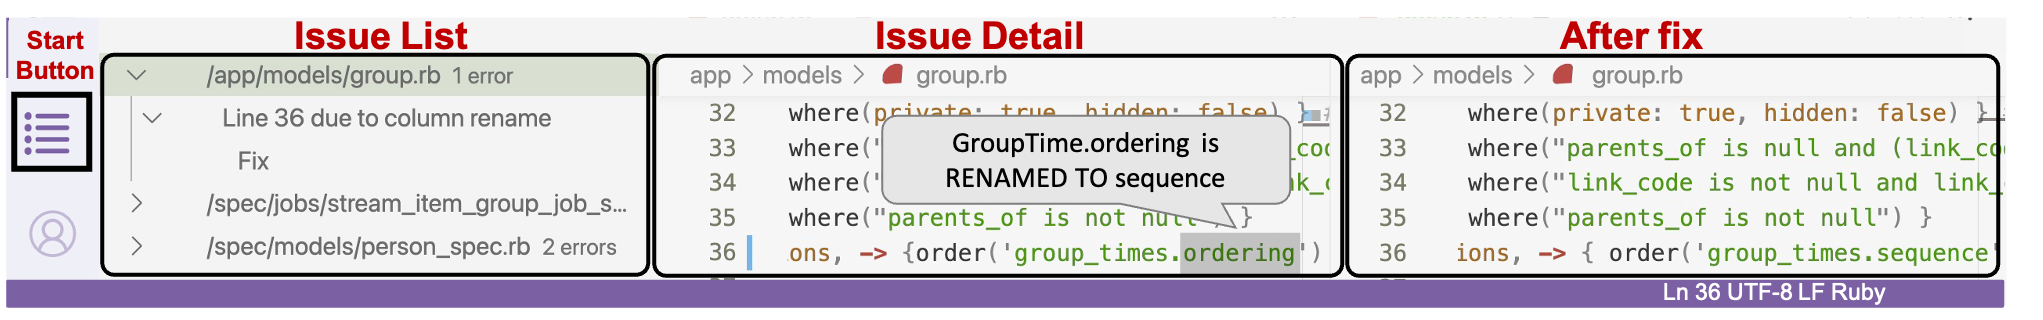
\includegraphics[width=\textwidth]{figs/plugin.png}
\caption{The screenshot of \Tool{} IDE Plugin}
\label{fig:vscode-plugin}
\end{figure*}


We have implemented \Tool{} as a plugin for Visual Studio Code~\cite{vscode}, a popular IDE for multiple languages.
% \shan{citation needed to back this claim up}
As shown in Figure~\ref{fig:vscode-plugin}, one can press the start button to start the plugin. By default, \Tool compares the current code with the latest commit.
% \shan{can I specify which commit to compare against? 
%If this is not difficult to implement, it would be nice to have}. 
Users can also specify the commits they desire to check in the configuration file. 

\textbf{Issue list.} The left panel, as shown in Figure~\ref{fig:vscode-plugin}, lists all the errors detected by \Tool in a hierarchical view. The first level lists
the files where errors are detected; clicking a file shows the details of every 
error in that file, including the line number and the type of root-cause schema change;
clicking the error shows a ``Fix'' button. 

\textbf{Issue detail.} Clicking a file in the issue list will navigate users to the corresponding file in the editor, with the error code highlighted. Users can hover their mouses over the highlighted code and see the detailed
explanation, like ``GroupTime.ordering is RENAMED TO sequence'' in Figure~\ref{fig:vscode-plugin}. 

\textbf{Issues fix.} One can click the  `\texttt{Fix}'  button  on the left panel
or a `\texttt{Fix all}' button to fix one or all the issues.


\subsection{Implementation}
The start button triggers our static analyzer to run on the given
code commits. The analyzer produces an \texttt{output.json} file that is parsed 
%by \texttt{getDepsInPackageJson} 
to create the issue list using  the Visual Studio Code Extension APIs \texttt{TreeDataProvider} and \texttt{TreeItem}. 
The \texttt{DocumentHighlightProvider} API is used to highlight the selected error code, given the filename and line number information in 
\texttt{output.json}. The \texttt{HoverProvider} API enables the tooltip of detailed reason to  display once hovering over the highlighted code.
To fix the error, \texttt{TextDocument}, \texttt{Range}, and  \texttt{ExtensionContext} APIs are used to insert, replace, and delete source code in the editor panel.





\section{Evaluation and Threats to Validity}
% \Tool{} can be downloaded from Visual Studio Marketplace~\cite{vscodemarketplace} and easily installed in Visual Studio Code. 

% % \shan{It is a bit strange to study 12 Rails apps in section 2, and only evaluate
% % 6 of them here. Better make them consistent.} 

% 


We have evaluated \Tool{} using \numRailsApp Ruby-on-Rails applications and \numDjangoApp Django applications (the same 12 applications described in
Section \ref{sec:back}). 
For each application, we apply \Tool{} on all its consecutive commits.  

\begin{table}
\caption{Inconsistency Detected by \Tool}
\label{tab:evaluation}
\centering
%\resizebox{0.8\columnwidth}{!}{
\begin{tabular}{lrrr}
\arrayrulecolor{black}\hline  
\arrayrulecolor{black}\hline
 & Rails  & Django  & Total\\
%\# of schema change & 12 & 23 & 35\\
\# of inconsistent queries & 38 & 48 & 86\\
%\# existing in release & 20 & 10 & 30\\
%\# of affected files & 26 & 31 & 57\\
\# of inconsistent queries in latest versions &  1 & 10 & 11\\
\# of inconsistent queries in past versions & 37 & 38 & 75\\
%Avg. (median) commits to fix past inconsis. & 576 (135) & 9 (8) & -\\
%Avg. (median) days to fix past inconsistency   &  378 (65) & 3 (3) & -\\
\arrayrulecolor{black}\hline  
\arrayrulecolor{black}\hline
\end{tabular}
%}
\end{table}


\textbf{Detection.} As shown in Table~\ref{tab:evaluation}. \Tool{} automatically identifies \numRailsError inconsistency errors caused by 35 schema changes, with no false positives based on our manual examination. Among them, 11 errors  exist in the latest versions. After reporting
them to developers,
10 already got confirmed. These 11 errors have existed for 234 days on average (median: 61 days) when reported by us. 
The other \numFixed errors on average existed in these applications
for 232 days (median: 7 days) and 409 commits (median: 16 commits)
until finally discovered and fixed by developers.
%took 378 days and 576 commits (median: 65 days and 135 commits)
%for Rails, and 3 days and 9 commits for Django developers
%to discover and fix. 
In theory, some developers may intentionally
split schema changes and follow-up code changes to separate commits.
This is unlikely for most of these errors given the long gap taken to fix
them.
Moreover, about half of them were not fixed until after major code releases.
%\numfixedafterrelease of them are fixed after the version is released.

%\junwen{There are only 9 patches for Rails and 5 patches for  Django  are exactly the same as what \Tool generates. For the rest, the error is fixed by removing either the whole query, whole function, or even the file.}

\textbf{Refactoring.} Among the 11 errors that we reported to developers, for 6
of them, developers already accepted the refactoring patches suggested by
\Tool and merged them into the main branch. For the other \numFixed errors that
were fixed by developers in the past, the related statements, functions, or files were
often deleted in the fixed commit. 
%\shan{TODO: not a surprise, because ...}
There are 13
of them where related code regions still existed in the fixed commit, and these 13 fixes are 
exactly the same as the refactoring suggested by \Tool. 

%Among these 35 schema changes, in the same commit the schema change is committed, developers already tried to change the corresponding code for 15 schema changes with \developerfixed queries in 35 files, which can also be automated by our tool. 
%\junwen{For developers' fix within the same commit, there are 9 patches for Rails and 18 patches for  Django  are exactly the same as what \Tool generates. }

 
% \shan{what exactly are these warnings?} caused by schema change and generates patches for \numRailsError of them (i.e., all but the index deletion change). We examined all of the detected errors and warnings and the suggested fixes, and found no false positives. And most of them are already fixed in their later versions\shan{a lot of explanation is needed here. readers may wonder
% whether you are simply detecting problems in an intermediate version that will not affect end
% users. It would also be helpful if I know how long it took for the problem to be fixed.}. 
% For those issues still exists in their latest versions \shan{how many are there in total?}, we have also reported 4 of them \shan{why do you only report 4?} to the issue tracking systems of these applications and 3 of them are already confirmed and merged. 

% \shan{you also need to comment on what are potential false negatives of your tool.}

\textbf{Performance.}
 \Tool{} takes 3--125 seconds (35s on average) to process consecutive commits of Rails applications with 11,000--900,000 lines of code, and 1--40 seconds (19s on average) for Django apps with 17,000--174,000 lines of code.  
% \shan{I noticed that you commented out the time information. I think it is necessary to just
% briefly report how long it takes for your analysis.}


\textbf{Threats to validity.}
As discussed in Section \ref{sec:approach}, 
\Tool may raise false alarms in rare cases.
%although we have not observed these cases in practice.
%Both Rails and Django allow developers to use special key words to declare non-persistent fields in a model class. In rare cases, a table column may be deleted from table, while a non-persistent field with the same name could be added to the same class. 
%Besides schema, it's possible for developers to define the classes' fields in multiple manners. For example Django allows using @property decorator on a function so that a class can use it as a field and Rails has similar API attr\_accessor. The application code that refers to those fields might be considered as inconsistent code incorrectly. We already tried our best to eliminate their influence in our tool design. But due to the flexibility of the languages, there might left some cases that our tool cannot handle.
%In addition to what already discussed in Section \ref{sec:approach}, 
There are also sources of false negatives.
%Firstly, the query extraction relies on type inference which only works within a file, it's possible to miss queries that are issued across files. Secondly, 
%the code parsing relies on existing parser libraries (pyparser for Django, and yard for rails), 
Application code that cannot be parsed by pyast or Yard cannot be analyzed by 
\Tool. A schema may be changed by SQL commands issued directly to the database
without any record in migration files. This is considered a bad  practice~\cite{migration-guide} and is not handled by \Tool.
A schema may also be changed in migration files 
through raw SQL commands wrapped in ORM APIs like
\texttt{migrations.RunSQL(...)} in
Django and \texttt{migrations.execute(...)} in Rails. 
This feature is rarely used by web developers (less than 1\% of cases in our study), and is not handled by \Tool.
If the new version adds a table \texttt{T}, and then changes the schema about 
\texttt{T} or its columns, indices, or
associations, \Tool would not check whether the new code is consistent with the
schema of \texttt{T}, as \texttt{T} does not exist in the old version.
Finally, what we observed in the 12 Rails and Django applications may not apply to
other open-source applications.

% \junwen{Why cannot we keep a record of functions with @property decorator, and remove the false positive}

% \junwen{Add the developers change code after schema change}
% \textbf{Django limitations.} Functions with the @property decorator that queries can refer to can create false positives for \Tool{}. For example, if a column is deleted but a function with an @property decorator that has the same name as that deleted column is created, \Tool{} will mark queries that refer to the function as queries that incorrectly refer to the schema. Thus, \Tool{} incorrectly raises these queries as errors because of the @property decorator (should I include an example). More generally, tables/columns/association relationships/indexes that are not recorded in an application’s migrations will not be included in the \Tool{}’s schema extraction and therefore there might be some false positives that arise. Annotations applied to a schema by a query in which the name of said annotation is the same as a deleted/renamed column can create false positives because that new annotation is not recorded in the extraction of the app’s schema. \Tool{} also requires python version >= 3.9.4 to be able to run.

% \shan{1. Can you offer some examples about the confirmed problems?
% 2. Please comment on the breakdown among rename vs. deletion vs. ... 
% }

% \begin{table}[ht!]
%     \centering
%     \caption{Evaluation result}
%     \resizebox{0.8\columnwidth}{!}{
%         \begin{tabular}{lrrrrr}
%         \hline
%           \hline
%          \# of issue & Table  & Column  & Association  & Index   \\
%         \hline
%         % \multicolumn{5}{l}{Rails Applications}\\
%         % \midrule
%         % Discourse & x & x & x & x  \\         
%         Lobster & 0 & 2 & 0 & 0 \\   
%         Gitlab & 0 & 1 & 0 &  2 \\   
%         % Redmine & x & x & x &  x \\   
%         Spree & 0 & 6 & 1 &  0 \\   
%         % Ror & 0 & 0 & 0 &  0 \\   
%         % Fulcrum & 0 & 0 & 0 &  0 \\   
%         Tracks & 0 & 4 & 4 &  0 \\   
%         Diaspora & 0 & 4 & 0 &  3 \\   
%         Onebody & 0 & 1 & 6 &  0 \\   
%         % Falling-fruit & 0 & 0 & 0 &  0 \\   
%         % Open street  & 0 & 0 & 0 &  0\\   
%         \hline
%         % \multicolumn{5}{l}{Django Applications}\\
%         % \midrule
%         Zulip & 0 & 2 & 0 & 0 \\   
%         Awx & 0 & 1 & 0 &  0 \\   
%         Saleor & 3 & 26 & 2 & 22 \\   
%         Healthchecks & 0 & 2 & 0 & 0 \\   
%         Gerapy & 0 & 1 & 0 & 0 \\   
%         Posthog & 5 & 0 & 0 & 0 \\   
%         \hline
%         Sum & 8 & 51 & 13 &  27 \\   
%         \hline
%         \hline
%         \end{tabular}
%     }
%     \label{tab:evaluation}
% \end{table}





\iffalse
\begin{table}[t!]
\caption{Developer's efforts}
\label{tab:effort}
\centering
%\resizebox{0.8\columnwidth}{!}{
\begin{tabular}{lrrr}
\arrayrulecolor{black}\hline  
\arrayrulecolor{black}\hline
 & Rails & Django & Sum \\
\# of schema change & 7 & 8 & 15\\
\# of affected queries & 28 & 63 & 91\\
\# of affected files & 16 & 31 & 47\\
\arrayrulecolor{black}\hline  
\arrayrulecolor{black}\hline
\end{tabular}
%}
\end{table}
\fi 


\input{evolutionsaver/Conclusion}
 